% $Header: /Users/joseph/Documents/LaTeX/beamer/solutions/conference-talks/conference-ornate-20min.en.tex,v 90e850259b8b 2007/01/28 20:48:30 tantau $

\documentclass{beamer}
\usepackage{siunitx}
\usepackage[font={footnotesize}]{caption}
\usepackage[
	backend=biber,
	style=authortitle,
	doi=false,
	% isbn=false, 
	maxcitenames=2,
]{biblatex}
\addbibresource{master.bib}

\definecolor{viridis_01}{rgb}{0.267004, 0.048740, 0.329415}
\definecolor{viridis_02}{rgb}{0.190631, 0.407061, 0.556089}
\definecolor{viridis_03}{rgb}{0.208030, 0.718701, 0.472873}
\definecolor{viridis_04}{rgb}{0.993248, 0.906157, 0.143936}

% \AtEveryCite{\color{viridis_03}}

% This file is a solution template for:

% - Talk at a conference/colloquium.
% - Talk length is about 20min.
% - Style is ornate.

% Copyright 2004 by Till Tantau <tantau@users.sourceforge.net>.
%
% In principle, this file can be redistributed and/or modified under
% the terms of the GNU Public License, version 2.
%
% However, this file is supposed to be a template to be modified
% for your own needs. For this reason, if you use this file as a
% template and not specifically distribute it as part of a another
% package/program, I grant the extra permission to freely copy and
% modify this file as you see fit and even to delete this copyright
% notice. 

\mode<presentation>
{
  % \usetheme{default}
  % \usecolortheme{beaver}
  \setbeamercolor{structure}{fg=viridis_01,bg=black!10!}
  % \setbeamercolor{palette secondary}{fg=viridis_02}

  % Remove figure prefix from figures.
  \setbeamertemplate{caption}{\insertcaption} 
}


\usepackage[english]{babel}
% or whatever

\usepackage[latin1]{inputenc}
% or whatever

% \usepackage{times}
\usepackage[T1]{fontenc}
\usepackage{graphics}
\usepackage{caption}
\usepackage{siunitx}
% Or whatever. Note that the encoding and the font should match. If T1
% does not look nice, try deleting the line with the fontenc.

\beamertemplatenavigationsymbolsempty
\usefonttheme{serif}

\title[Short title] % (optional, use only with long paper titles)
{
    Modeling Extracellular Potentials of Pyramidal Neurons and Interneurons%
}

% \subtitle
% {
% }

\author % (optional, use only with lots of authors)
{Daniel M. Bj\o rnstad}
% - Give the names in the same order as the appear in the paper.
% - Use the \inst{?} command only if the authors have different
%   affiliation.

\date{June 10, 2016}

\institute
{
    Master Thesis Summary
}




% If you have a file called "university-logo-filename.xxx", where xxx
% is a graphic format that can be processed by latex or pdflatex,
% resp., then you can add a logo as follows:

% \pgfdeclareimage[height=0.5cm]{university-logo}{university-logo-filename}
% \logo{\pgfuseimage{university-logo}}



% Delete this, if you do not want the table of contents to pop up at
% the beginning of each subsection:
%
%\AtBeginSubsection[]
%{
  %\begin{frame}<beamer>{Outline}
  %  \tableofcontents[currentsection,currentsubsection]
  %\end{frame}
%}


% If you wish to uncover everything in a step-wise fashion, uncomment
% the following command: 

%\beamerdefaultoverlayspecification{<+->}


\begin{document}

\begin{frame}
  \titlepage
\end{frame}

%\begin{frame}{Outline}
%  \tableofcontents
  % You might wish to add the option [pausesections]
%\end{frame}


% Structuring a talk is a difficult task and the following structure
% may not be suitable. Here are some rules that apply for this
% solution: 

% - Exactly two or three sections (other than the summary).
% - At *most* three subsections per section.
% - Talk about 30s to 2min per frame. So there should be between about
%   15 and 30 frames, all told.

% - A conference audience is likely to know very little of what you
%   are going to talk about. So *simplify*!
% - In a 20min talk, getting the main ideas across is hard
%   enough. Leave out details, even if it means being less precise than
%   you think necessary.
% - If you omit details that are vital to the proof/implementation,
%   just say so once. Everybody will be happy with that.

% Overview:
%   Motivation and conclusion is very important.
%   This is the first time there have been multiple models of  
%   extracellular potentials have been compared.
%   
%   
% - State the problem?
%       Measuring are often done using tetoredes
% - Goals
%       What can many models of extracellular potentials tell us.
%       Spike width and amp. have been used. Which definition is best.
% - The effects of filtering.
%       Drastically changes spike shape but seperation between neurons can still be seen.
%
% Pictures:
% - Many spikes around a neuron in a grid.
% - Blue brain article

\begin{frame}{Classifying Neurons Based On EAP}
    \begin{itemize}
        \item Extracellular action potentials (EAP) are unique for each neuron.
        \item Was early recoqnized that some interneurons had faster spikes than pyramidal
            neurons. 
        \begin{figure}
            \centering
            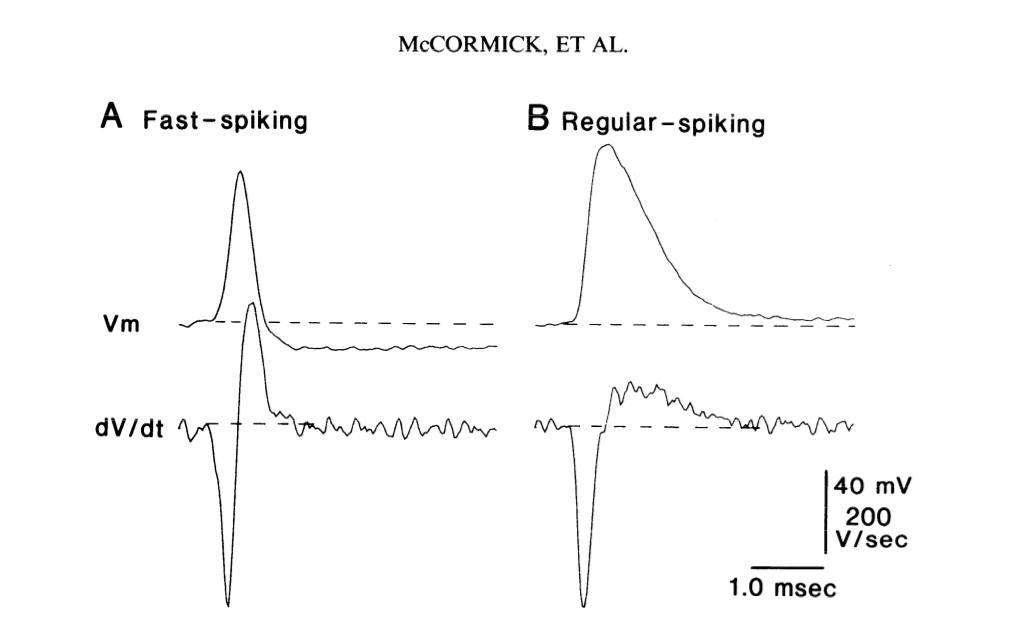
\includegraphics[height=0.5\textheight]{images/mc_cormick_fs_rs.png}\\
        \end{figure}
    \end{itemize}
\end{frame}

\begin{frame}{Motivation}
    \begin{itemize}
        \item More and more models allow simulations of EAP.
        \item One of the first times EAP simulations of different neurons have been compared.
        \item Many definitions of spike width and amplitude, some might be better suited
            for classification than others.
    \end{itemize}
\end{frame}

\begin{frame}{Methods: Model of the Cell Membrane}
    \centering
    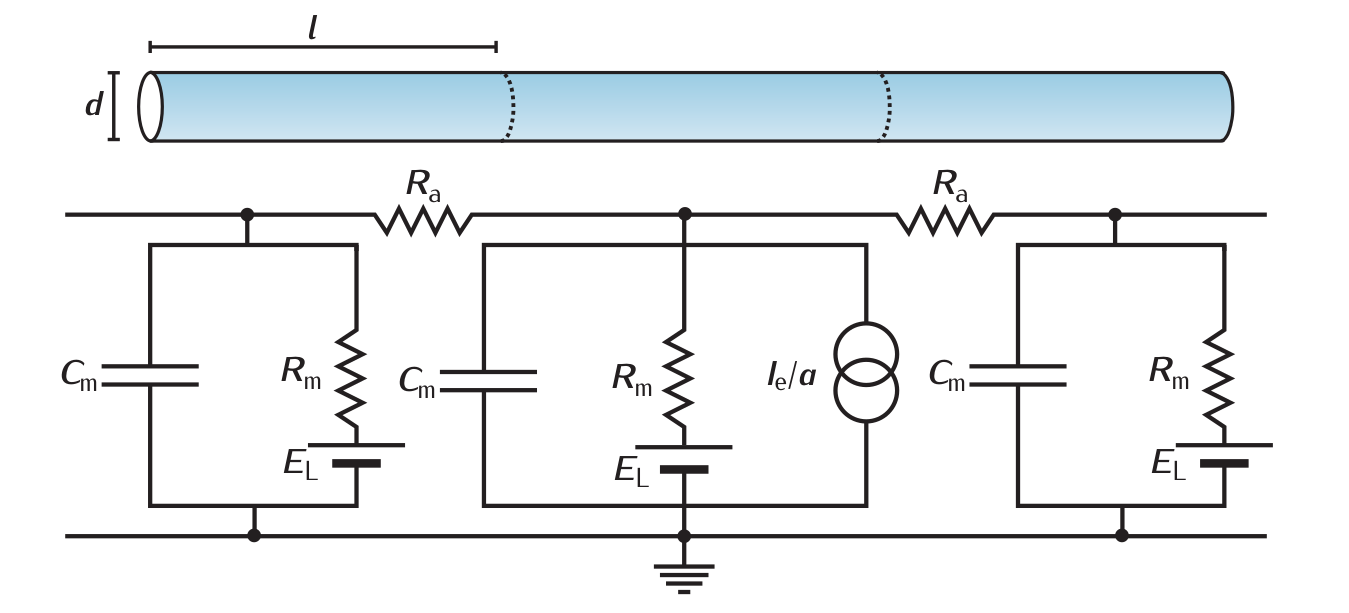
\includegraphics[width=\textwidth]{images/compartment_circuit.png}
\end{frame}

\begin{frame}{Compartmental Models}
    \centering
    Simulations can be done with NEURON.
    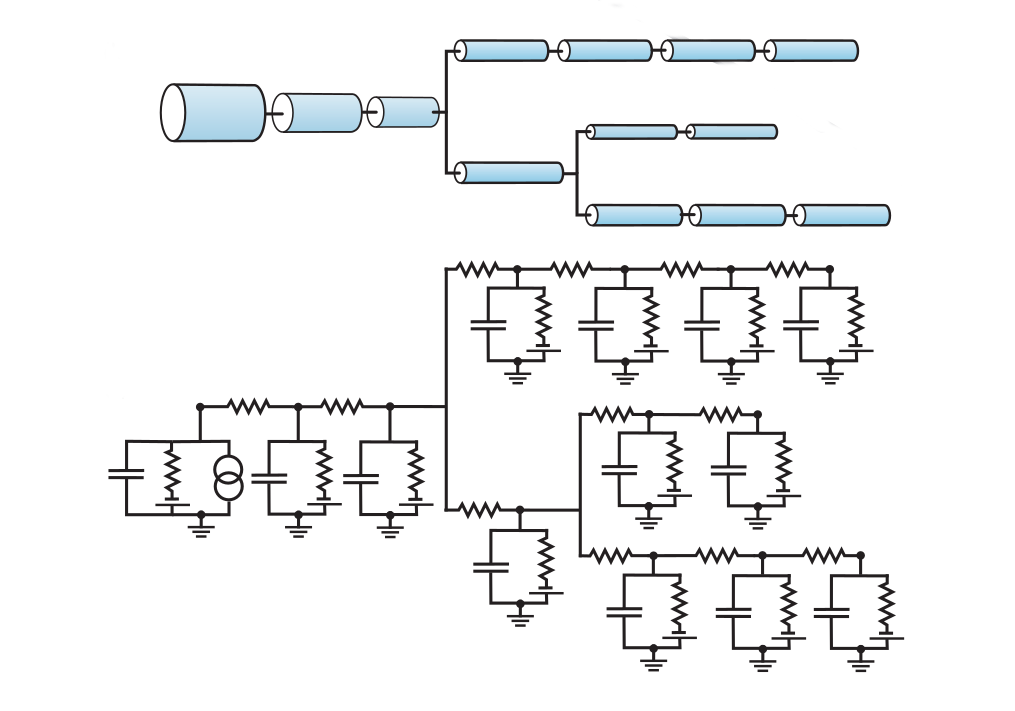
\includegraphics[width=\textwidth]{images/compartment_circuit_big.png}

\end{frame}

\begin{frame}{Calculation of Extracellular Potential}
    \begin{itemize}
        \item The potential generated by transmembrane currents.
    \end{itemize}
    % \centering
    $$\Phi(r,t) = \frac{1}{4\pi\sigma} \sum_{i=1}^n \frac{I_i(t)}{r_i} $$
    \begin{itemize}
        \item This is implemented in the python package LFPy.
        \item Results have been created using NEURON, LFPy and LFPyUtil.
    \end{itemize}
    % This is implemented in the python package LFPy.
    % Results have been created using NEURON, LFPy and LFPyUtil.
\end{frame}

\begin{frame}{Conservation of Current}
    Kirchhoff's current law: All transmembrane currents must sum to 0.
    \centering
    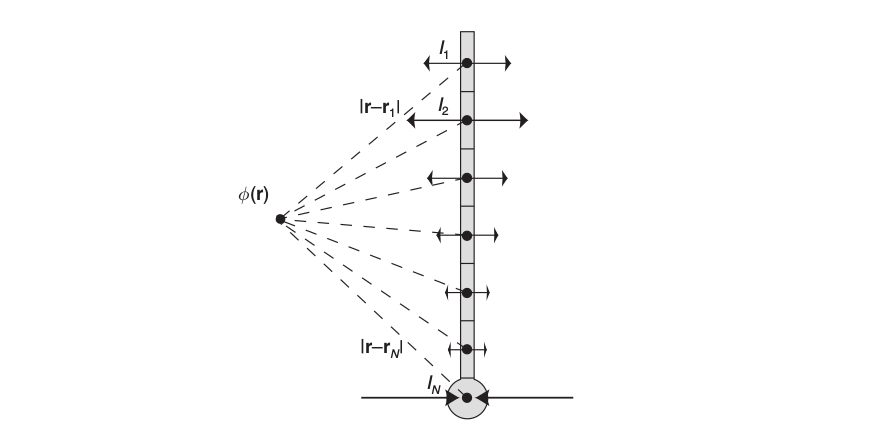
\includegraphics[width=\textwidth]{images/kirchhoff_current.png}
\end{frame}

\begin{frame}{Blue Brain Neuronal Microcircuit}
    % L5 P14 male Wistar Han rats. Seperated into morphological and 
    % electrophysiological types
    % I am using models from the blue brain team. Who are they, where are they. 
    % What rats, which area. L5 because of lots of research there.
    \centering
    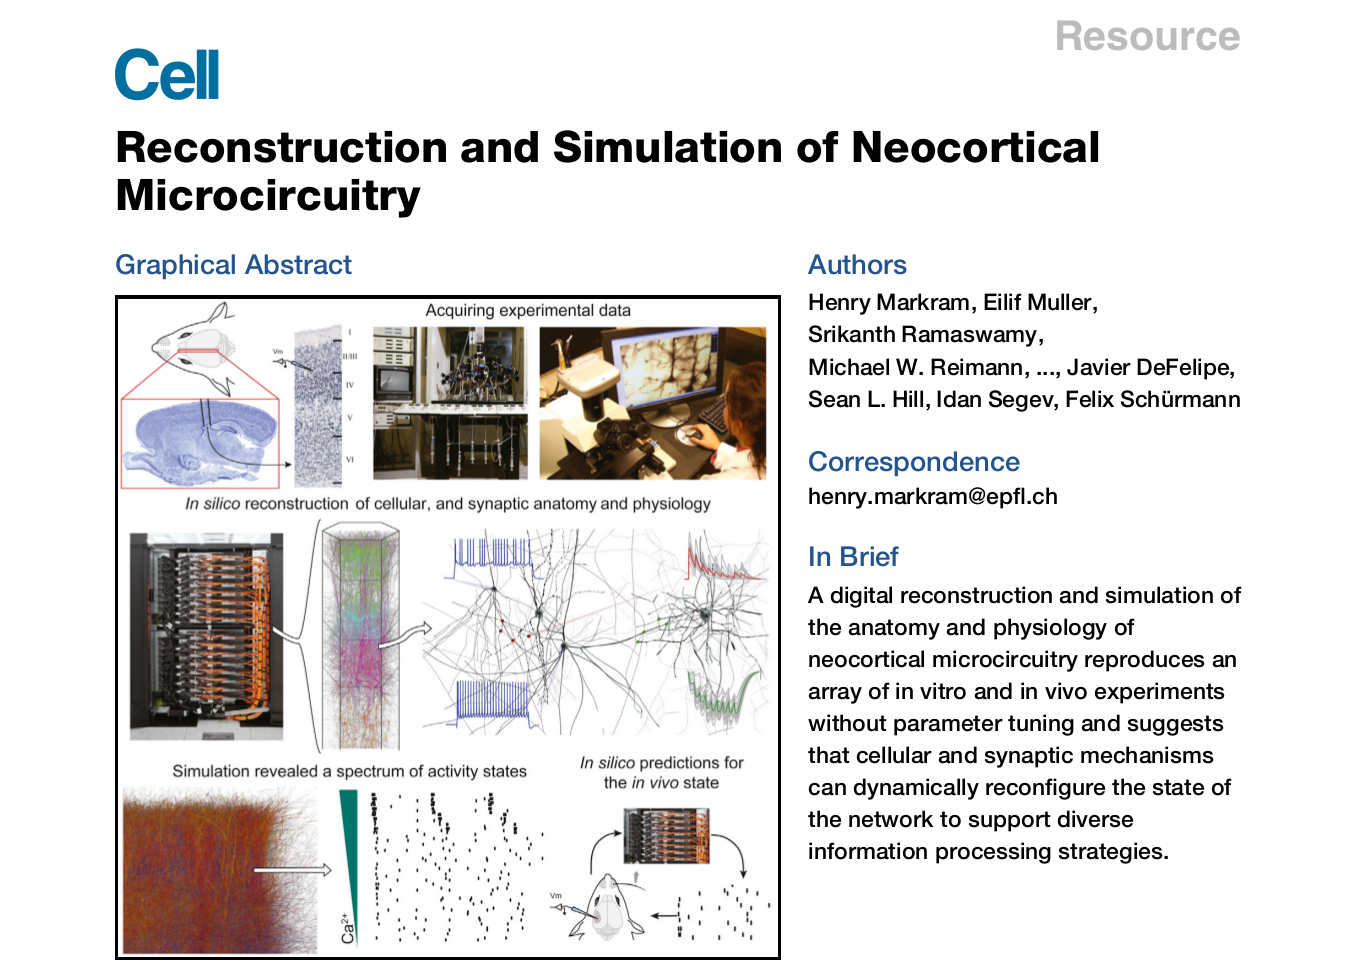
\includegraphics[width=\textwidth]{images/markram_front.png}
\end{frame}

\begin{frame}{Blue Brain Neuron Models}
    % Show the m-types.
    \begin{figure}
        \centering
        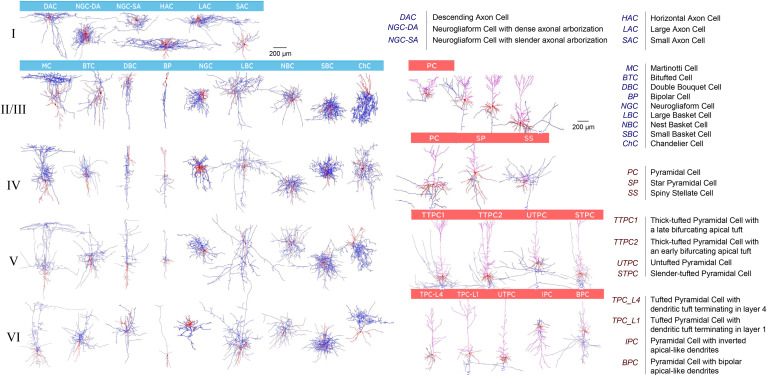
\includegraphics[width=\textwidth]{images/m-types.jpg}\\
        % \caption{\centering Fig. 2 in \textcite{markram_reconstruction_2015}}
    \end{figure}
\end{frame}

\begin{frame}{Blue Brain Neuron Models}
    % Show the e-types.
    \begin{figure}
        \centering
        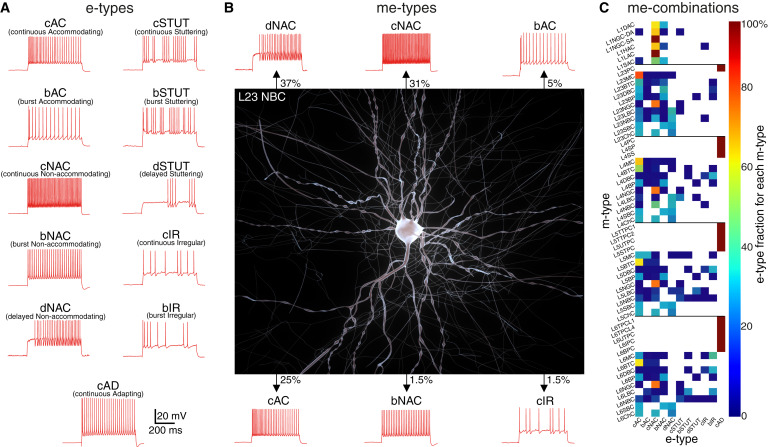
\includegraphics[width=\textwidth]{images/e-types.jpg}\\
        % \caption{\centering Fig. 4 in \textcite{markram_reconstruction_2015}}
    \end{figure}
\end{frame}

\begin{frame}{Selected Blue Brain Models}
    \begin{itemize}
        \item TTPC1, TTPS2, STPC, UTPC - Pyramidal neurons with different morphology, 
            but same e-type.
        \item LBC - cAC, cNAC, dSTUT, bAC - Similar morphology, different e-type.
        \item NBC - cNAC, dSTUT, bAC, bIR - Similar morphology, different e-type.
    \end{itemize}
\end{frame}

\begin{frame}{Results: Running a Simulation}
    \centering
    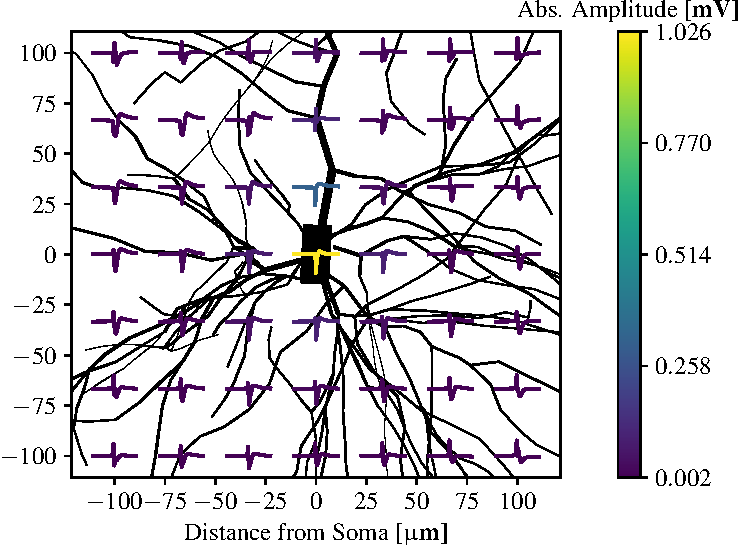
\includegraphics[width=\textwidth]{images/grid_y_x_signals_2d_normalized.pdf}
\end{frame}

\begin{frame}{Sources Spike Variability}
    \begin{itemize}
        \item Location of electrode.
        \item Inter spike interval.
        \item Bursting behavior.
        \item Backproagating action potentials.
        \item Synaptic input, position and shape.
        \item Filtering.
    \end{itemize}
% Factors that change action potentials width:
% * Firing frequency.
% * Input current. Higher current gives higher frequency.
% * Number of previous spikes.
% * Bursting behavior.
% * Backproagating action potentials.
% EAP:
% * Where the synaptic input is.
% * Filtering effects.
\end{frame}

\begin{frame}{Imitating Placement of Electrodes}
    500 electrodes positioned at random locations within 60 \si{\micro\metre} for 
    each selected model.
    % Show a pyramidal neuron from the simulation with electrodes and a arrow to a spike.
    \centering
    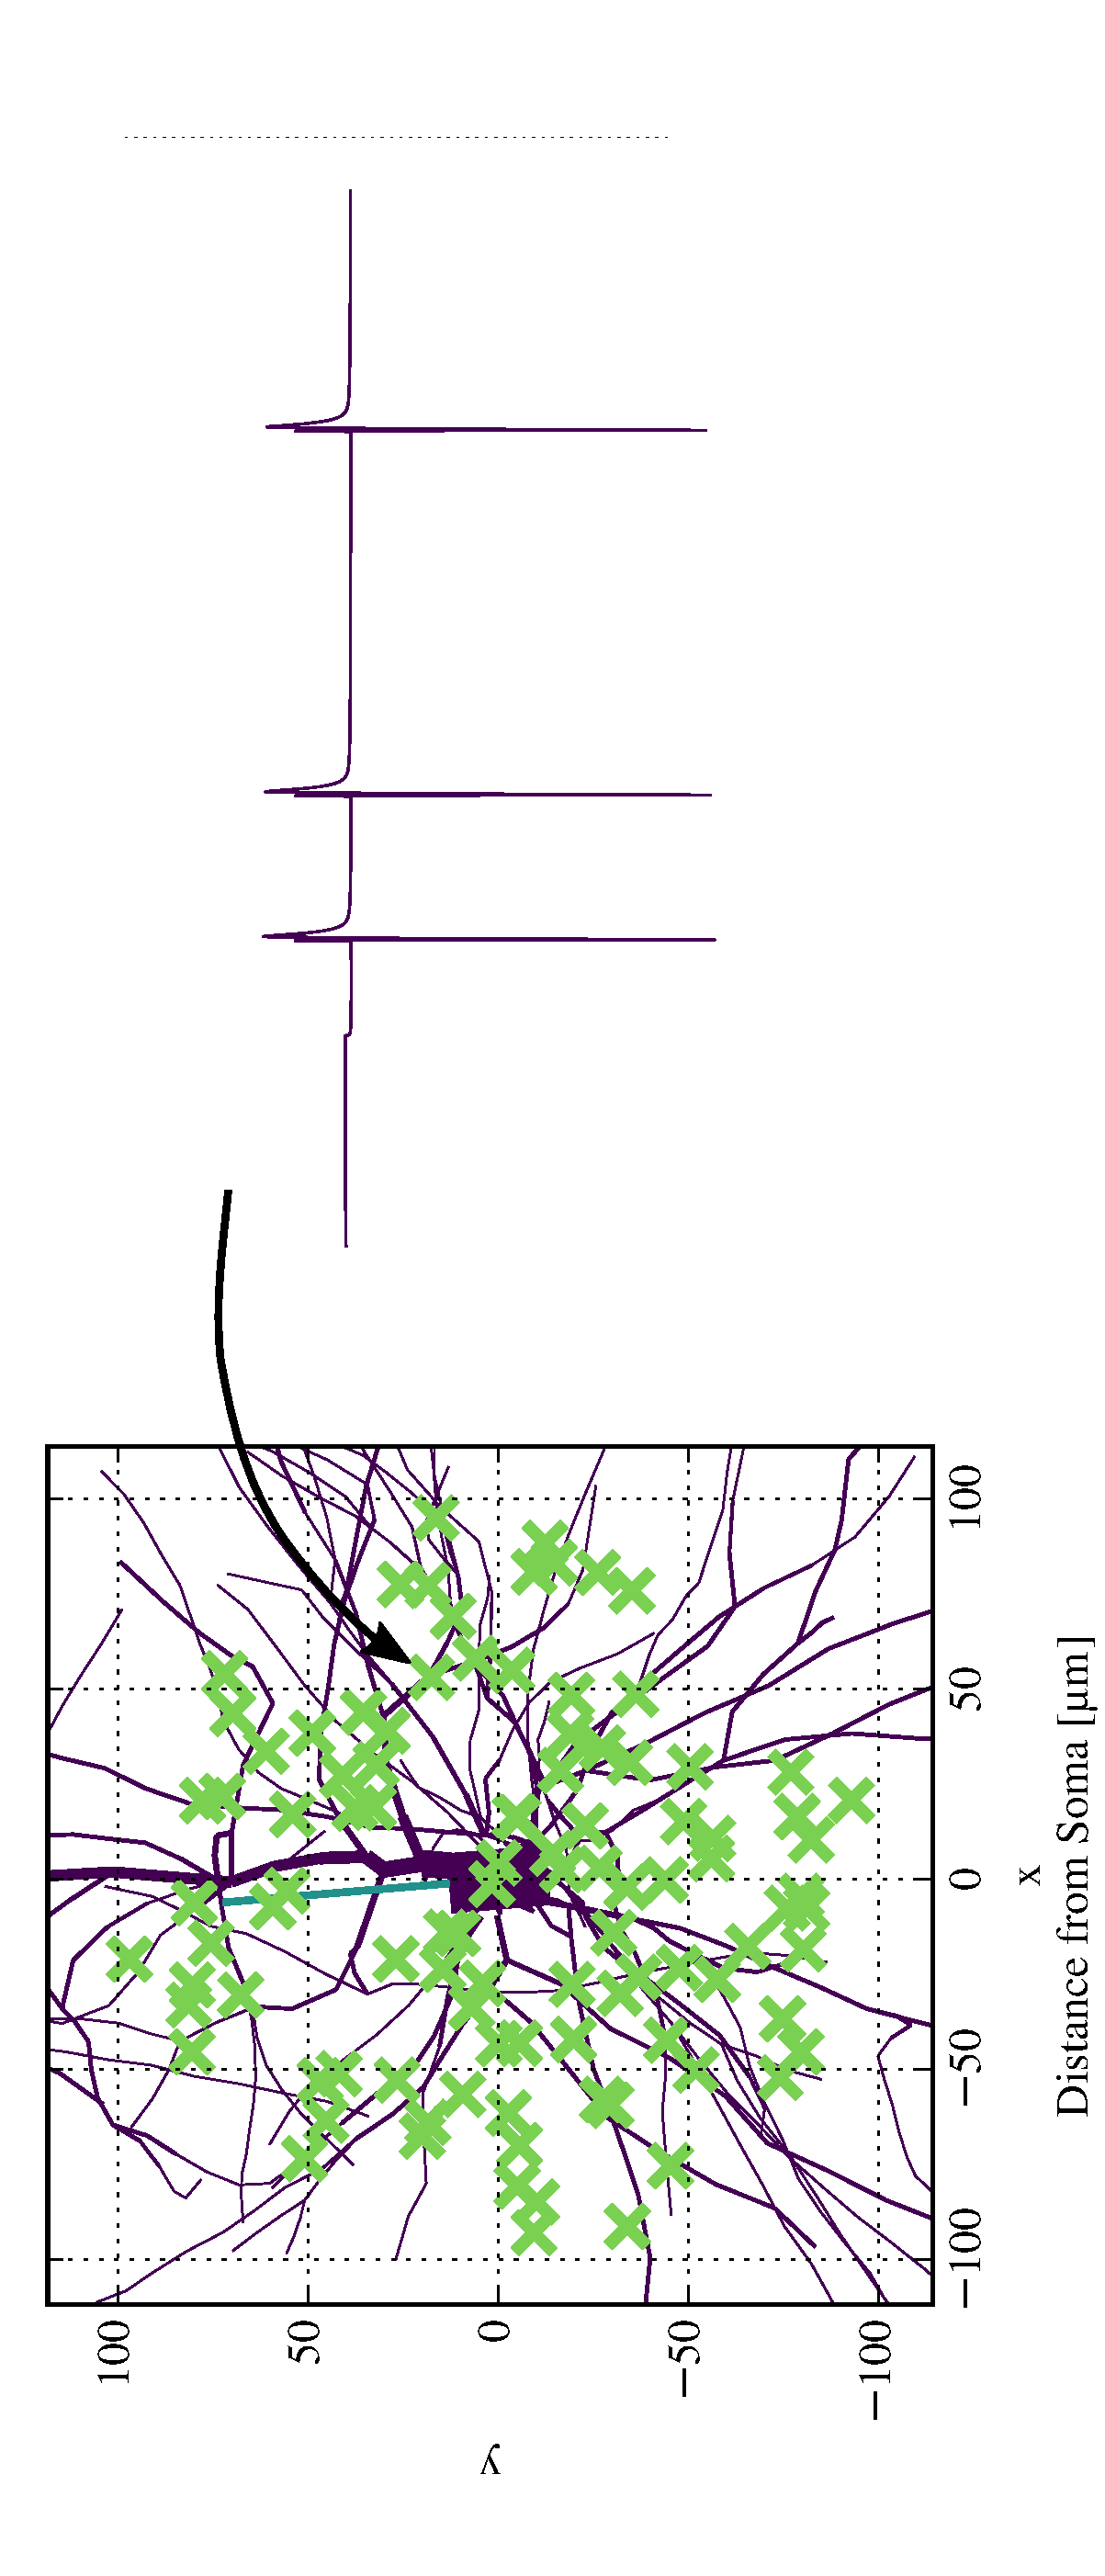
\includegraphics[angle=-90,width=\textwidth]{images/electrodes.pdf}
\end{frame}

\begin{frame}{Spike Width Definition}
    \centering
    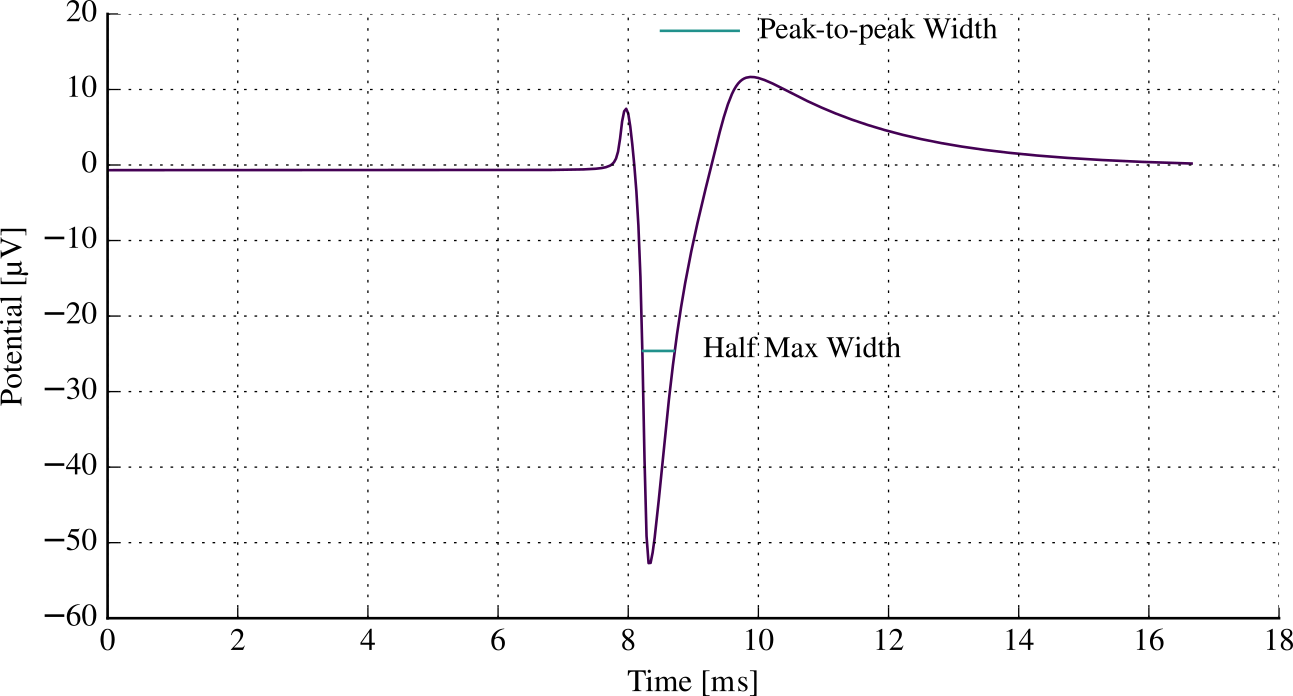
\includegraphics[width=\textwidth]{images/width_good.png}
\end{frame}

\begin{frame}{Effect of Spike Width Definition}
    % Which definiton gives the better seperation. 
    % Peak to peak gives better seperation knowing the distance from soma.
    % Peak to peak has better variance compared
    \centering
    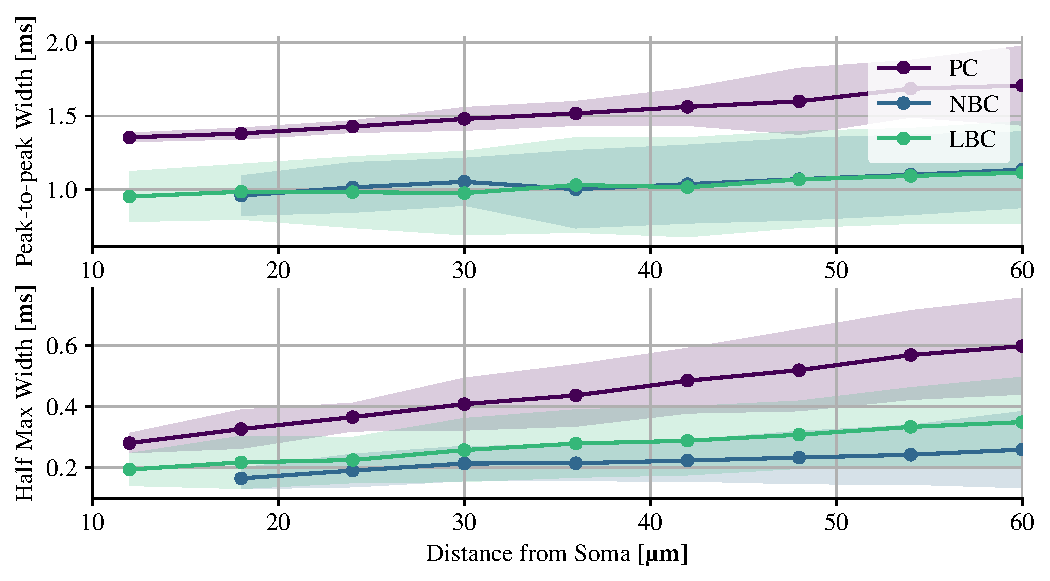
\includegraphics[width=\textwidth]{images/TTPC2_NBC_LBC_widths.pdf}
\end{frame}

\begin{frame}{Spike Amplitude Definition}
    % % Zoom in on the spike. Show two common definitions, width at half maximum and peak to peak width.
    % Peak-to-peak and half maximum width definitions.
    % \centering
    % 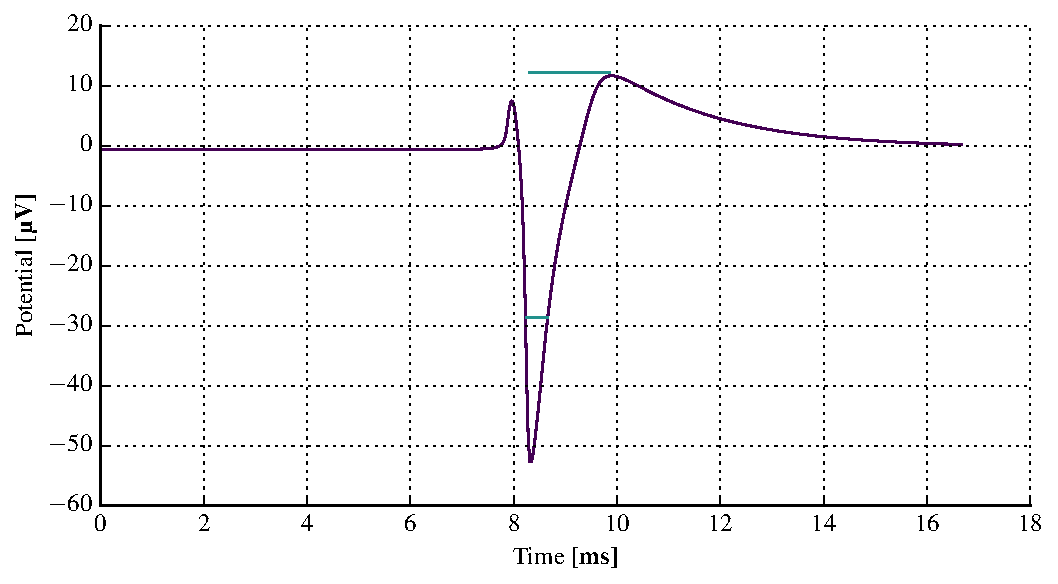
\includegraphics[width=\textwidth]{images/widthdef_extracellular_1.pdf}
    % Zoom in on the spike. Usually two definitons used, peak to peak, baseline.
    % Show them.
    Peak-to-peak and baseline-to-peak amplitude.
    \centering
    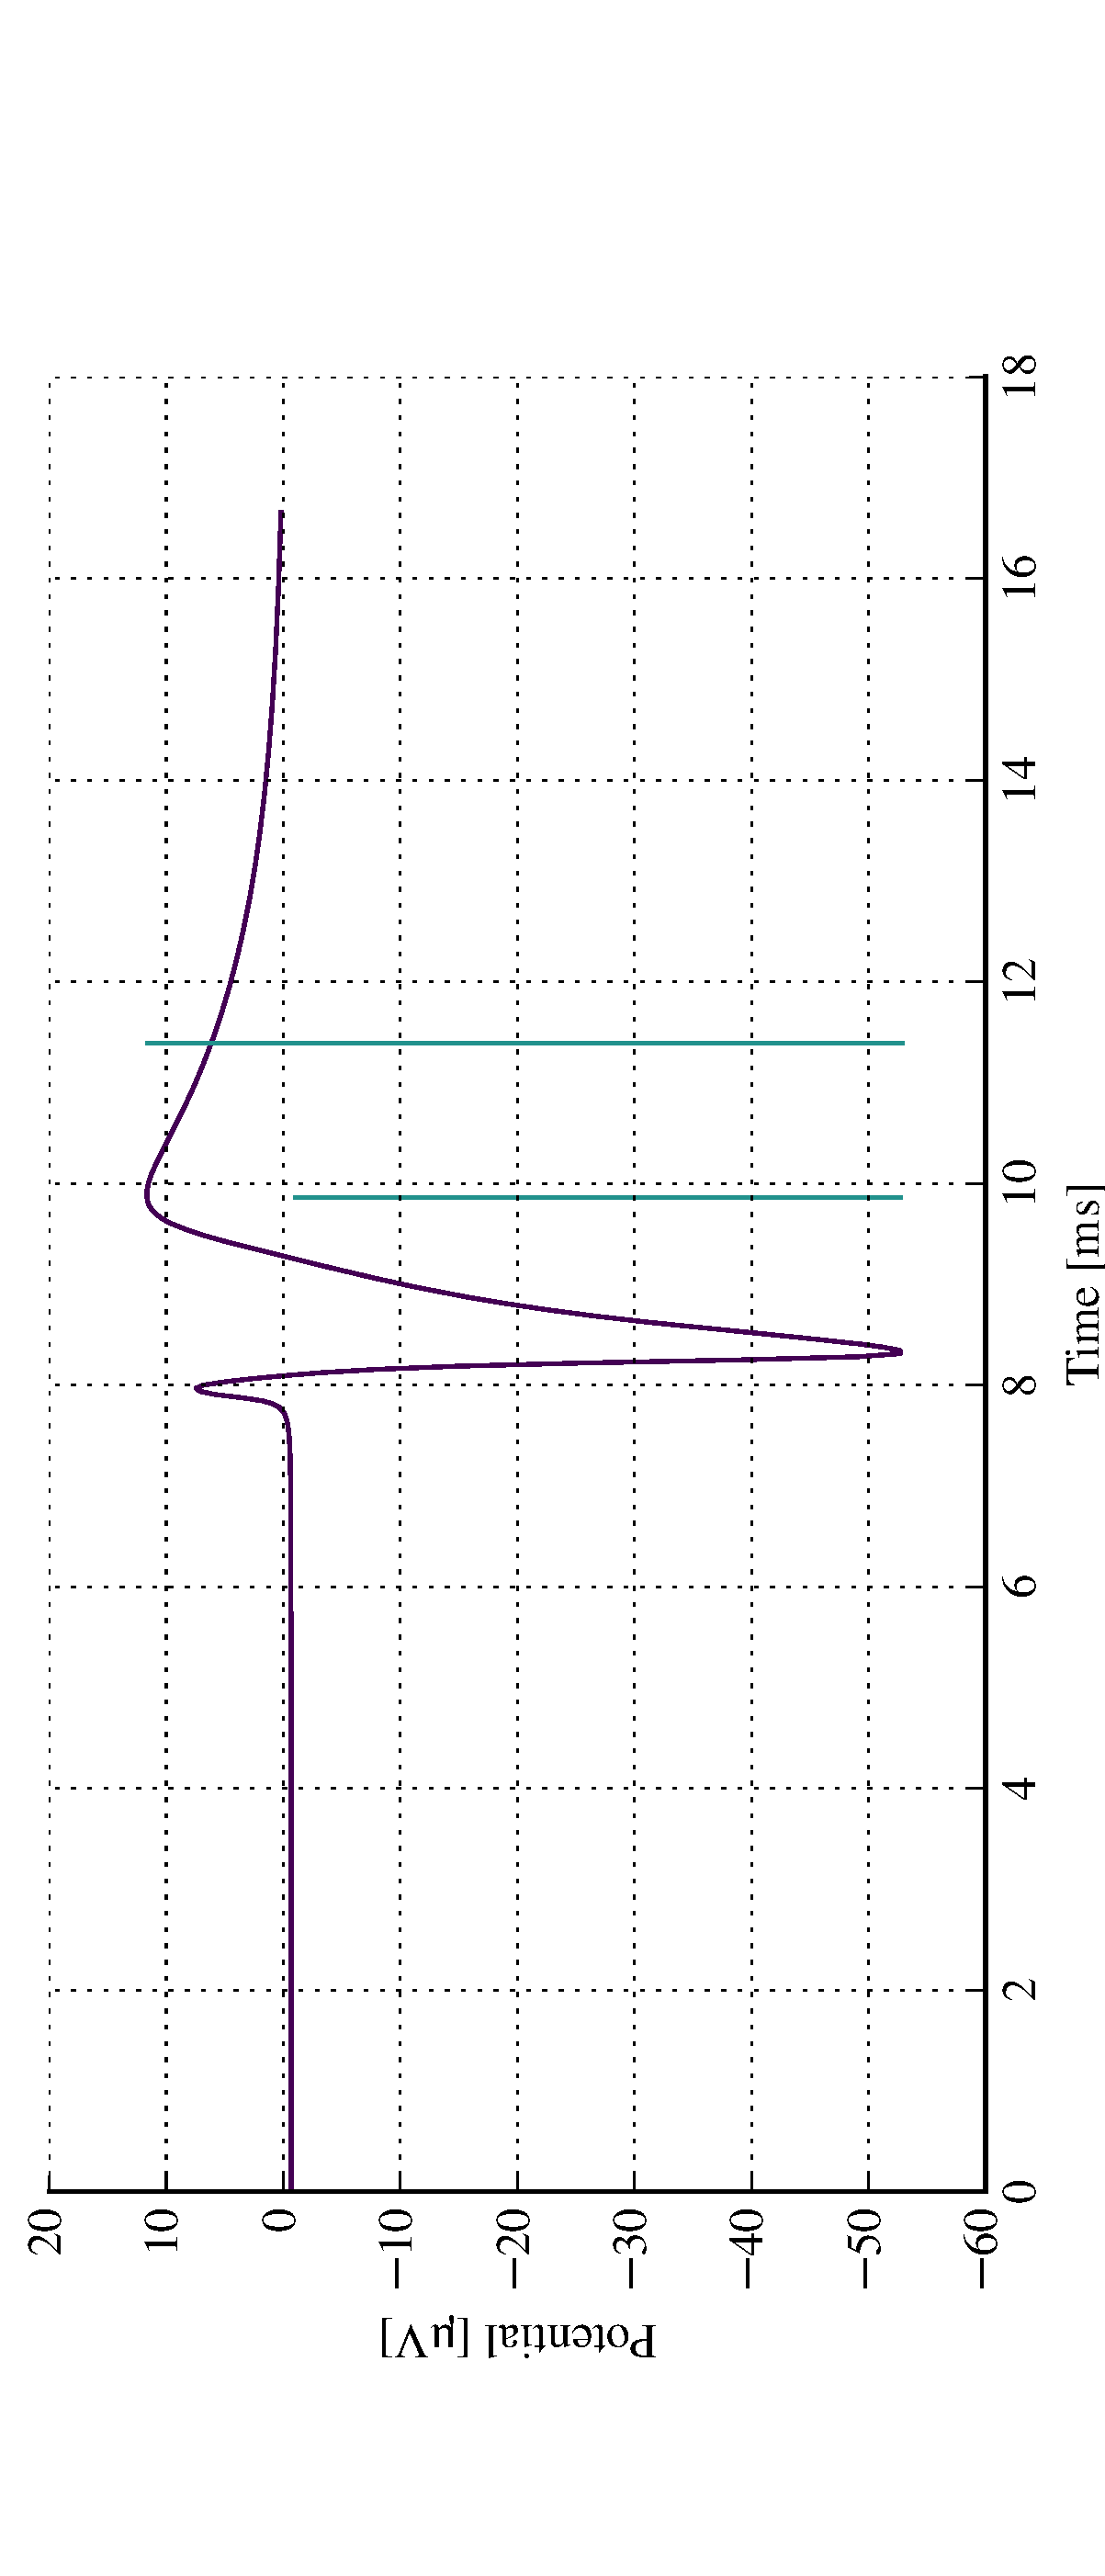
\includegraphics[angle=-90,width=\textwidth]{images/amp_def.pdf}
\end{frame}

\begin{frame}{Effect of Spike Amplitude Definition}
    % Introduce the models, why they were chosen. Not very interesting.
    % What is a good definition? The seperation is good, but for all distances.
    % Heavy overlap for inhib types. But good seperation between the types.
    % Points closer to soma has fewer samples. 
    \centering
    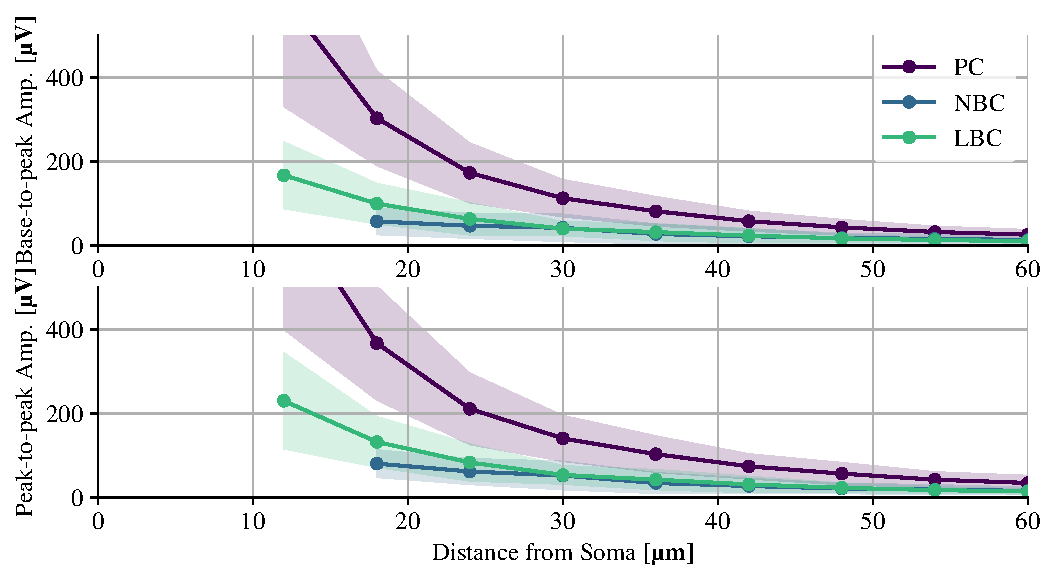
\includegraphics[width=\textwidth]{images/TTPC2_NBC_LBC_amps.pdf}
\end{frame}

\begin{frame}{Neuronal Classification}
    % Variation in interneurons are much bigger than with the pyramidal models.
    % Might be because of the models, not sure if this is a feature of the models or 
    % the neurons.
    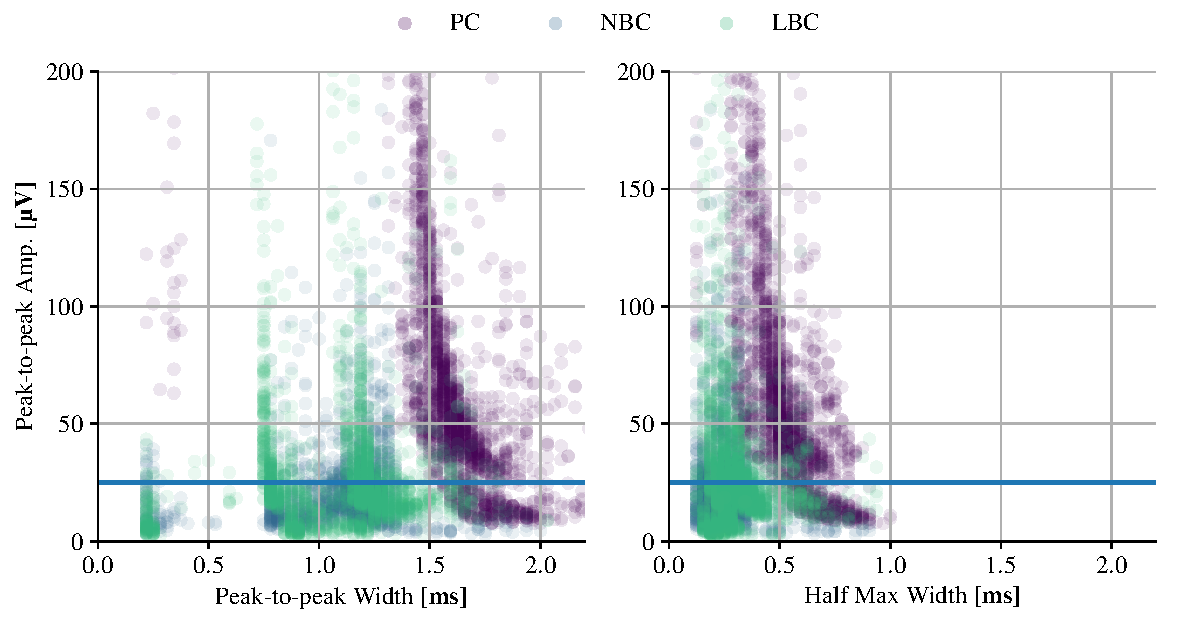
\includegraphics[width=\textwidth]{images/TTPC2_NBC_LBC_IN_combined_scatter.pdf}
\end{frame}

\begin{frame}{Neuronal Classification}
    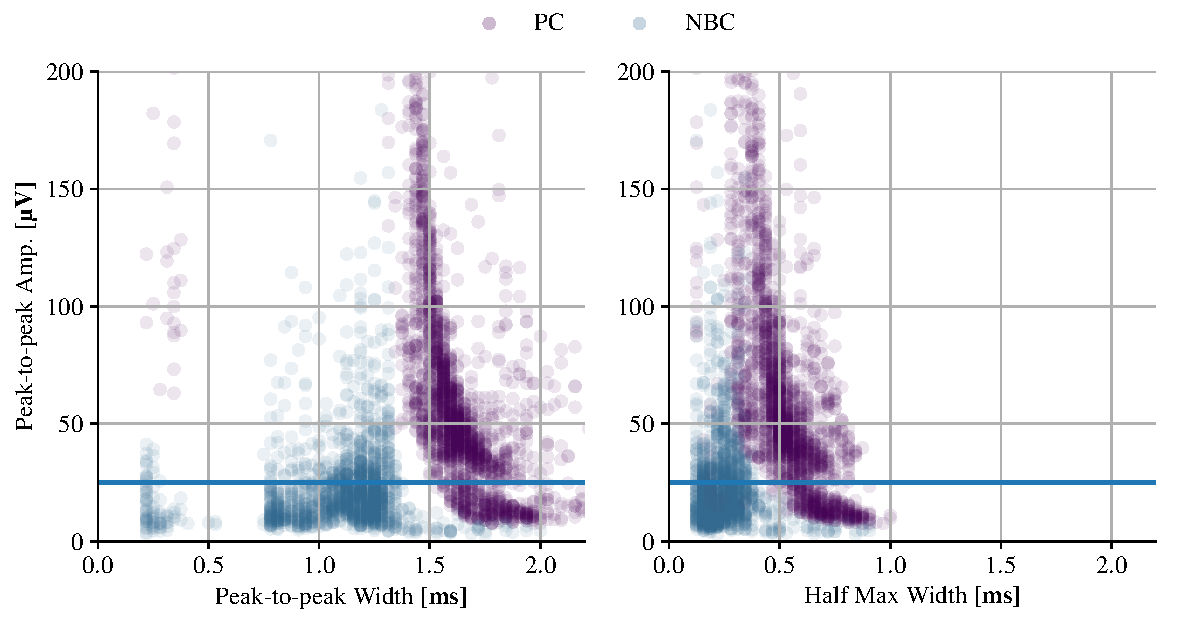
\includegraphics[width=\textwidth]{images/TTPC2_NBC_scatter.pdf}
\end{frame}

\begin{frame}{Neuronal Classification}
    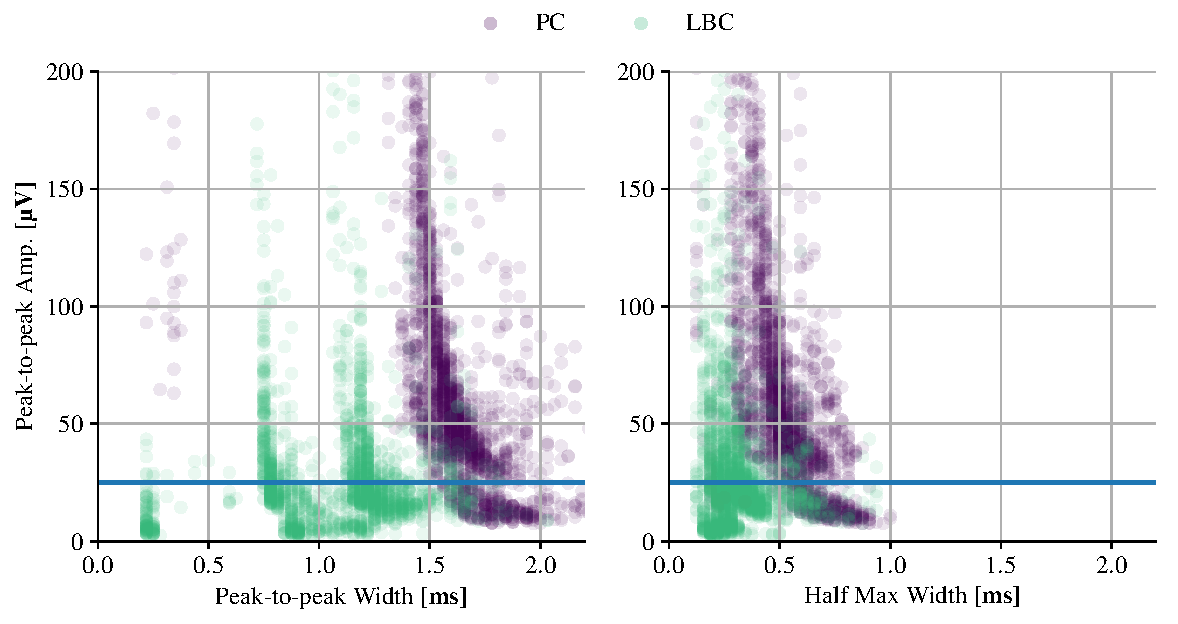
\includegraphics[width=\textwidth]{images/TTPC2_LBC_scatter.pdf}
\end{frame}

% \begin{frame}{Comparing Width Definitions}
%     Other remarks:
%     \begin{itemize}
%         \item Baseline is not always well defined.
%         \item Peak-to-peak more resistant to noise.
%         \item Half width requires high temporal resolution.
%         \item Widths seem a bit long compared to other experimental results.
%     \end{itemize}
% \end{frame}


\begin{frame}{Conclusion}
    Summary:
    \begin{itemize}
        % \item Models are in compliance with experimental results.
        \item Peak-to-peak definition of width gives better measurements.
        \item Amplitude should be considered when classifying based on width.
        \item If the theory holds, tetrode measurements can identify some neuronal classes
            based on spike amplitude and width.
        \item The newly developed simulation environment LFPyUtil allows quick
            convertion to EAP calculation for new models.
    \end{itemize}
    % Remarks:
    % \begin{itemize}
    %     \item Width was not used by blue brain, inter spike interval more commonly used recently.
    % \end{itemize}
\end{frame}

\end{document}
